\documentclass[
  final,
  babelLanguage=italian,
  %desktopVersion,
  %showtrims,
  %overleaf,
]{anecdote}

\graphicspath{{./assets/images/}}

% Page size: 6x9 inch
% Body text: 10.5 / 15 pt

\usepackage{local}

%% Details of the book
%% ===================

\title{Il Conoscere è Adesso}
\subtitle{}
\author{Ajahn Sumedho}
\publisher{Edizioni Santacittarama}
\date{2017-08-21}
\editionInfo{\emph{Prima edizione}, 5.000 copie, stampate in Malesia, 2018}
\ISBN{978-88-85706-03-3}

% === Metadata ===

\pdfinfo{%
  /Title (\thetitle)%
  /Author (\theauthor)
  /Subject (meditation)
  /Keywords (buddhism, Dhamma, meditation)
  /GTS_PDFXVersion (PDF/X-1:2001)%
  /GTS_PDFXConformance (PDF/X-1a:2001)%
}

%% === Load further packages ===

%% === Hyphenation exceptions and corrections ===

\hyphenation{London}

\begin{document}

\frontmatter

\ifdesktopversion
\desktopCover{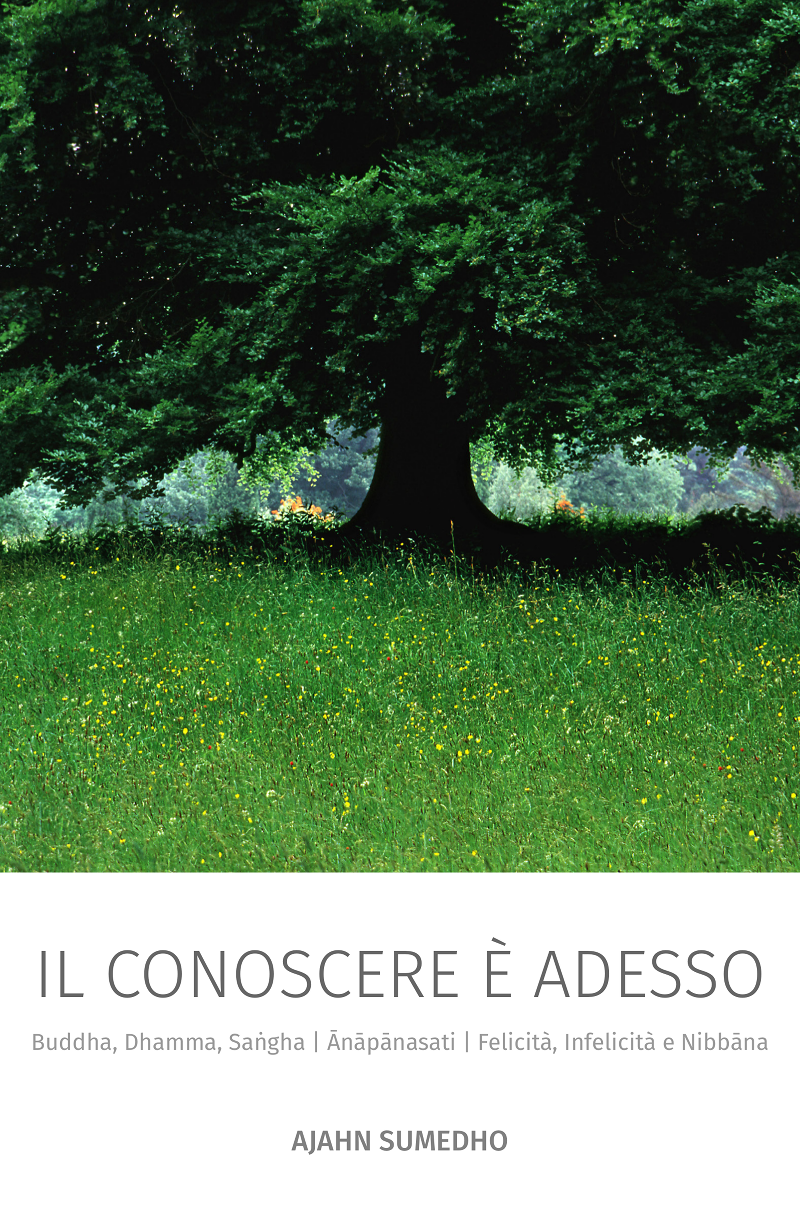
\includegraphics[height=\paperheight]{./desktop-cover.png}}
\fi

% FIXME: convert to CMYK jpg

\cleartoverso
\thispagestyle{empty}
\mbox{}
\AddToShipoutPicture*{\put(\LenToUnit{0.85in},\LenToUnit{5.5in}){%
    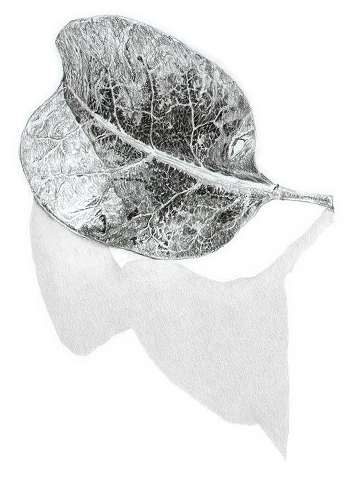
\includegraphics[width=30mm,keepaspectratio]{spearshape_by_Scott_edited.png}%
}}

\cleartorecto
\thispagestyle{empty}

{\raggedleft
\firaSansLightFont
\color[gray]{0.35}%

\vspace*{4\baselineskip}
\setlength{\parskip}{1em}
\setlength{\parindent}{0pt}

{\fontsize{22}{25}\selectfont
\color[gray]{0.3}%
\MakeUppercase{\thetitle}}

\vspace*{0.9\baselineskip}

{\fontsize{12}{15}\selectfont
\theauthor}

\vfill

Pubblicato per la distribuzione gratuita da\\
EDIZIONI SANTACITTARAMA

{\fontsize{9}{12}\selectfont
Questo libro può essere scaricato gratuitamente dal sito web:}

\vspace*{-0.8\baselineskip}%
{\fontsize{9}{12}\selectfont
www.fsbooks.org}%

}



\cleartoverso
\thispagestyle{empty}

{\copyrightsize
\centering
\setlength{\parindent}{0pt}%
\setlength{\parskip}{0.8\baselineskip}%

% --- TODO format copyright info

Pubblicato per la distribuzione gratuita da

EDIZIONI SANTACITTARAMA

Questo libro può essere scaricato gratuitamente dal sito web:

\href{http://www.forestsangha.org/}{\emph{www.fsbooks.org}}

IL CONOSCERE È ADESSO

di Ajahn Sumedho

Pubblicato da:

Edizioni Santacittarama,

Monastero Santacittarama, 02030 Poggio Nativo RI, Italia

www.santacittarama.org

Traduzione di Donatella Levi

Foto di copertina di Chinch Gryniewicz

Copyright © 2018 ASSOCIAZIONE SANTACITTARAMA

ISBN: 978-88-85706-03-3

Questo libro può essere scaricato gratuitamente dal sito web:
\href{http://www.forestsangha.org/}{\emph{\emph{www.fsbooks.org}}}

\emph{Sabbadanam dhammadanam jinati}

``Il dono del Dhamma supera tutti i doni''

Titolo originale:

NOW IS THE KNOWING

Pubblicato da Aruno Publications, Regno Unito
(\href{http://www.ratanagiri.org.uk/}{\emph{www.ratanagiri.org.uk}})

Copyright © 2011 Harnham Buddhist Monastery Trust

Questo lavoro è autorizzato da Creative Commons

Attribution-NonCommercial-NoDerivs3-0 Unported License

\emph{https://creativecommons.org/licenses/by-nc-nd/2.0/uk/}

V. pag ??? per maggiori dettagli su diritti e restrizioni

Prima edizione, 5.000 copie, stampate in Malesia, 2018

% ---

\thetitle\ -- \thesubtitle\\
by \theauthor

Published by \thePublisher

ISBN \theISBN

Copyright \copyright\ \thePublisher\ 2017

Cover Photograph: The Person

\vfill

{\footnotesize

This work is licensed under a Creative Commons\\
Attribution-NonCommercial-NoDerivatives 4.0 International~License.

Produced with the \LaTeX\ typesetting system, set in Gentium and Crimson Roman.

\theEditionInfo

}}


\cleartorecto
\thispagestyle{empty}

\mbox{}\vfill

\vspace*{-2\baselineskip}

\begin{verse}

{\itshape
``Il passato è un ricordo.\\
Il futuro è l'ignoto.\\
Il conoscere è adesso.''}
\bigskip

{\upshape\fontsize{9}{12}\selectfont
\MakeUppercase{Ajahn Sumedho}}

\end{verse}

\vfill\mbox{}

\clearpage
\thispagestyle{empty}

\mbox{}\vfill

{\centering
Vogliamo esprimere la nostra gratitudine per l'aiuto ricevuto da molte
persone nella preparazione di questo libro, in particolare al gruppo
Kataññuta della Malesia, Singapore e Australia, per averne reso
possibile la stampa.
\par}

\vfill\mbox{}

\cleartorecto
\tableofcontents*

% Page 1 is the first page of the first chapter.
\mainmatter

\chapter{Buddha, Dhamma, Saṅgha}

Quando le persone ci chiedono: ``Cosa è necessario fare per diventare
buddhisti?'', rispondiamo che abbiamo preso rifugio nel Buddha, nel
Dhamma, nel Saṅgha. E per prendere rifugio recitiamo una formula in
lingua pāḷi:

\emph{Buddhaṃ saranaṃ gacchāmi}

\emph{Prendo rifugio nel Buddha}

\emph{Dhammaṃ saranaṃ gacchāmi}

\emph{Prendo rifugio nel Dhamma}

\emph{Saṅghaṃ saranaṃ gacchāmi}

\emph{Prendo rifugio nel Saṅgha.}

Man mano che procediamo nella pratica, e cominciamo a realizzare la
profondità degli insegnamenti buddhisti, prendere questi rifugi diventa
una vera gioia - anche solo recitarli è fonte di ispirazione per la
mente. Sono monaco da ventidue anni, eppure mi piace ancora recitare
``\emph{Buddhaṃ saranaṃ gacchāmi}'', a dire il vero ancor più di quanto
non mi piacesse ventuno anni fa. All'epoca, infatti, queste parole non
avevano per me alcun significato, le intonavo perché dovevo farlo,
perché faceva parte della tradizione. Prendere rifugio nel Buddha
semplicemente a livello verbale non vuole affatto dire che si stia
prendendo rifugio in qualcosa: anche un pappagallo potrebbe essere
addestrato a dire ``\emph{Buddhaṃ saranaṃ gacchāmi}'', e questo avrebbe
per lui altrettanto poco significato quanto lo ha per molti buddhisti.
Queste parole sono intese perché ci si rifletta sopra, perché le si
osservi e ci si interroghi sul loro significato: cosa vuol dire
``rifugio'', cosa vuol dire ``Buddha''? Quando diciamo: ``Prendo rifugio
nel Buddha'', cosa intendiamo? Come possiamo utilizzare tutto questo in
modo che non sia un insieme ripetuto di sillabe prive di senso, ma
qualcosa che ci aiuta davvero a ricordare, a darci una direzione, ad
accrescere la nostra devozione e dedizione al sentiero del Buddha?

La parola ``Buddha'' è una parola meravigliosa, significa ``colui che
conosce'', e il primo rifugio è nel Buddha in quanto personificazione
della saggezza. Una saggezza non personificata risulta per noi troppo
astratta: non siamo capaci di concepire una saggezza priva di corpo,
priva di anima, e così, poiché la saggezza sembra avere sempre una
qualità personale, utilizzare il Buddha come suo simbolo è molto utile.

Possiamo usare la parola Buddha per riferirci a Gotama, il fondatore di
quello che oggi è noto come buddhismo, il saggio storico che raggiunse
il \emph{Parinibbāna} in India 2.500 anni fa, colui che insegnò le
Quattro Nobili Verità e l'Ottuplice Sentiero, insegnamenti da cui
traiamo beneficio ancor oggi. Tuttavia, quando prendiamo rifugio nel
Buddha non vuol dire che stiamo prendendo rifugio in un qualche profeta
storico, ma in ciò che vi è di saggio nell'universo, nelle nostre menti,
in ciò che non è separato da noi ma che è più reale di qualsiasi cosa si
possa concepire con la mente o di cui si possa fare esperienza
attraverso i sensi. Senza una ``saggezza-di-Buddha'', sarebbe
assolutamente impossibile una vita di una qualche durata nell'universo;
è la ``saggezza-di-Buddha'' che protegge. Noi la chiamiamo
``saggezza-di-Buddha'', altri possono utilizzare termini diversi -- in
fin dei conti si tratta solo di parole, e noi utilizziamo quelle della
nostra tradizione. Non litigheremo sulle parole pāḷi, sulle parole
sanscrite, o su quelle ebraiche, greche, latine, inglesi o di altro tipo
- stiamo solo usando l'espressione ``saggezza-di-Buddha'' come simbolo
convenzionale che ci aiuti a ricordare di essere saggi, di essere
vigili, di essere svegli.

Nel nord-est della Thailandia molti monaci della foresta usano la parola
``Buddho'' come oggetto di meditazione. La utilizzano come una sorta di
\emph{koan}. Prima calmano la mente seguendo le inspirazioni e le
espirazioni usando le sillabe BUD-DHO, poi iniziano a contemplare:
``Cosa è Buddho, `colui che conosce'? Cosa è il conoscere?''.

Quando andavo in \emph{tudong} (errare a piedi) percorrendo il nord-est
della Thailandia mi piaceva fermarmi presso il monastero di Ajahn Fun.
Ajahn Fun era un monaco molto amato e profondamente rispettato,
l'insegnante della Famiglia Reale, ed era così popolare che riceveva
ospiti in continuazione. Io mi sedevo presso la sua \emph{kuṭī}
(capanna) e lo stavo ad ascoltare mentre teneva alcuni dei suoi
straordinari discorsi di Dhamma, tutti incentrati sul tema ``Buddho'' --
da quanto potevo capire, insegnava solo questo. Riusciva a trasformare
questa pratica in una meditazione davvero profonda, adatta sia a un
contadino analfabeta che a un aristocratico thailandese elegante ed
educato all'occidentale. La parte principale del suo insegnamento non
consisteva nel ripetere solo meccanicamente ``Buddho'', ma nel
riflettere e investigare, nel risvegliare la mente a osservare in
profondità ``Buddho'', ``colui che conosce'', investigando realmente il
suo inizio e la sua fine, sopra e sotto, così che la propria attenzione
vi aderisse completamente. Quando si faceva così, la parola ``Buddho''
diventava qualcosa che risuonava nella mente. La si investigava, la si
osservava, la si esaminava, prima di pronunciarla e dopo averla
pronunciata, e a un certo punto si cominciava ad ascoltarla, e a sentire
al di là del suono, fino a quando si sentiva il silenzio.

Un rifugio è un luogo in cui si è al sicuro, e così quando delle persone
superstiziose si recavano dal mio maestro Ajahn Chah chiedendogli
medaglioni avvolti da incantesimi o piccoli talismani che li
proteggessero da proiettili, coltelli, fantasmi e così via, lui
rispondeva: ``Perché volete queste cose? La sola vera protezione è
prendere rifugio nel Buddha. Prendere rifugio nel Buddha è
sufficiente''. Ma di solito la loro fede nel Buddha non era altrettanto
forte di quella in questi sciocchi medaglioni. Loro volevano qualcosa di
bronzo o di creta, timbrato e benedetto. Questo vuol dire prendere
rifugio nel bronzo e nella creta, prendere rifugio nella superstizione,
prendere rifugio in ciò che è davvero insicuro e non ci può essere
realmente d'aiuto.

Al giorno d'oggi nella Gran Bretagna moderna le persone sono in genere
più sofisticate, non prendono rifugio negli amuleti magici, prendono
rifugio in cose come la Westminster~Bank - ma anche questo vuol dire
prendere rifugio in qualcosa che non offre alcuna sicurezza. Prendere
rifugio nel Buddha, nella saggezza, significa avere un luogo sicuro.
Quando c'è la saggezza, quando agiamo saggiamente e viviamo saggiamente,
siamo realmente al sicuro. Le condizioni intorno a noi potrebbero
cambiare, non abbiamo alcuna garanzia su quale sarà il tenore di vita, o
se la Westminster Bank supererà questo decennio. Il futuro rimane
sconosciuto e misterioso, ma nel presente, prendendo rifugio nel Buddha,
abbiamo la presenza mentale che ci consente di riflettere sulla vita e
imparare da essa mentre la viviamo.

Saggezza non vuol dire conoscere tante cose sul mondo; non abbiamo
bisogno di andare all'università e raccogliere informazioni sul mondo
per essere saggi. Saggezza vuol dire conoscere la natura delle
condizioni mentre ne facciamo esperienza. Non consiste nel farsi
catturare e assorbire per forza d'abitudine dalle condizioni dei nostri
corpi e delle nostre menti, reagendo condizionati dalla paura, dalla
preoccupazione, dal dubbio, dall'avidità e così via, ma vuol dire usare
quel ``Buddho'', ``colui che conosce'', per osservare che queste
condizioni sono mutevoli. È proprio l'atto del conoscere quel
cambiamento ciò che chiamiamo Buddha e in cui prendiamo rifugio. Non
abbiamo la pretesa che quel Buddha sia ``me'' o ``mio''. Non diciamo
``Io sono Buddha'', ma piuttosto ``Prendo rifugio nel Buddha''. È un
modo per sottomettersi umilmente a quella saggezza, essendo consapevoli,
essendo svegli.

Benché in un certo senso prendere rifugio sia qualcosa che facciamo
continuamente, la formula pāḷi che utilizziamo è un richiamo per la
memoria, perché dimentichiamo, perché prendiamo abitualmente rifugio
nella preoccupazione, nel dubbio, nella paura, nella rabbia,
nell'avidità e così via. L'immagine del Buddha ha una funzione simile;
quando ci inchiniamo di fronte ad essa non immaginiamo che sia qualcosa
di diverso da un'immagine di bronzo, un simbolo. È un modo di riflettere
che ci rende un po' più consapevoli del Buddha, del nostro rifugio nel
Buddha, nel Dharma, nel Saṅgha. L'immagine del Buddha siede con grande
calma e dignità, non in trance ma pienamente vigile, con uno sguardo
colmo di consapevolezza e gentilezza, non scalfita dalle condizioni
mutevoli intorno ad essa. Sebbene l'immagine sia fatta di bronzo, mentre
noi abbiamo questi corpi di carne e sangue, e quindi per noi è molto più
difficile, pur tuttavia è un richiamo. Alcune persone assumono un
atteggiamento bigotto rispetto alle immagini del Buddha, ma qui in
Occidente non ho trovato che costituiscano un pericolo. I veri idoli in
cui crediamo e che veneriamo, e che ci ingannano continuamente, sono i
nostri pensieri, le nostre opinioni e convinzioni, i nostri amori e odi,
la nostra arroganza e presunzione.

Il secondo rifugio è nel Dhamma, nella verità ultima o realtà ultima. Il
Dhamma è impersonale; non cerchiamo in alcun modo di personificarlo, di
trasformarlo in una qualche sorta di deità personale. Quando recitiamo
in pāḷi il verso sul Dhamma, diciamo che esso è ``\emph{sandihiṭṭhiko
akāliko ehipassiko opanayiko paccattaṃ veditabbo viññūhi}''. Dato che il
Dhamma non ha attributi personali, non possiamo nemmeno dire che sia
buono o cattivo, o dotato di qualsiasi altra qualità superlativa o di
paragone: esso è al di là delle concezioni dualistiche della mente.

Perciò quando descriviamo il Dhamma o vi alludiamo lo facciamo
attraverso parole come ``\emph{sandihiṭṭhiko}'', che vuol dire
immanente, qui-e-ora. Questo ci riporta al presente; avvertiamo un senso
di immediatezza, di attualità. Si potrebbe pensare che il Dhamma sia un
qualcosa che è ``là fuori'', qualcosa da ricercare altrove, ma
\emph{sandihiṭṭhikodhamma} vuol dire che è immanente, qui-e-ora.

\emph{Akālikadhamma} significa che il Dhamma non è vincolato da alcuna
condizione temporale. La parola \emph{akāla} significa senza tempo. La
nostra mente concettuale non è in grado di concepire qualcosa che sia
senza tempo, perché le nostre concezioni e percezioni sono condizioni
basate sul tempo, però ciò che possiamo dire è che il Dhamma è
\emph{akāla}, non condizionato dal tempo.

\emph{Ehipassikadhamma} è un richiamo ad andare a vedere, a volgersi o
dirigersi verso il Dhamma. Vuol dire guardare, essere consapevoli. Non è
che preghiamo il Dhamma di venire, o aspettiamo che ci batta sulla
spalla; dobbiamo impegnarci attivamente. È come nel detto di Gesù:
``Bussate e vi sarà aperto''. \emph{Ehipassiko} vuol dire che dobbiamo
mettere in atto lo sforzo di volgerci verso la verità.

\emph{Opanayiko} vuol dire che porta verso l'interiorità, verso la pace
all'interno della mente. Il Dhamma non ci spinge verso ciò che è
affascinante o eccitante, verso le romanticherie o l'avventura, ma
conduce al Nibbāna, alla calma, al silenzio.

\emph{Paccattaṃ veditabbo viññūhi} vuol dire che possiamo conoscere il
Dhamma solamente attraverso l'esperienza diretta. È come il sapore del
miele, se lo assaggia qualcun altro continueremo a non conoscerne il
sapore. Potremmo conoscerne la formula chimica, o essere in grado di
recitare tutto ciò che di poetico è stato scritto sul miele, ma solo
quando lo assaggeremo personalmente sapremo davvero com'è. È lo stesso
con il Dhamma: dobbiamo assaggiarlo, dobbiamo conoscerlo direttamente.

Prendere rifugio nel Dhamma vuol dire prendere un altro rifugio sicuro.
Non si prende rifugio in una filosofia o in concetti intellettuali, in
teorie, idee, dottrine o credenze di qualche tipo. Non ci rifugiamo in
una credenza nel Dhamma, o in Dio, o in qualche forza là fuori nello
spazio, oppure in qualcosa che è ``al di là'' o è separato, qualcosa che
dovremo incontrare prima o poi nel futuro. Le descrizioni del Dhamma ci
tengono ancorati al presente, nel qui e ora libero da vincoli temporali.
Prendere rifugio è un modo di riflessione immediato, immanente nella
mente; non consiste nel ripetere come pappagalli ``\emph{Dhammaṃ saraṇaṃ
gacchāmi}'', pensando ``I buddhisti dicono così per cui lo devo dire
anch'io''. Noi ci volgiamo verso il Dhamma, siamo consapevoli adesso,
prendiamo rifugio nel Dhamma adesso, come un'azione immediata, un
riflesso immediato dell'essere il Dhamma, essere quella stessa verità.

La nostra mente, nel suo elaborare continuamente concetti, tende sempre
a fuorviarci, portandoci nel divenire. Pensiamo: ``Praticherò la
meditazione così un giorno mi illuminerò. Prenderò i Tre Rifugi per
diventare buddhista. Voglio diventare saggio. Voglio sfuggire alla
sofferenza e all'ignoranza ed essere diverso''. Questa è la mente
concettuale, la mente desiderante, la mente che ci trae sempre in
inganno. Invece di pensare continuamente secondo la prospettiva del
divenire in futuro qualcosa, prendiamo rifugio nell'essere Dhamma nel
presente.

L'impersonalità del Dhamma costituisce un problema per molte persone,
perché la religione devozionale tende a personificare tutto, e chi viene
da questo tipo di tradizioni non si sente a suo agio se non in una
qualche forma di relazione personale. Ricordo che un giorno un
missionario cattolico francese venne nel nostro monastero per praticare
la meditazione. Si trovò un po' in difficoltà con l'approccio buddhista,
perché disse che era come una ``gelida operazione chirurgica'', non
c'era una relazione personale con Dio. Non si può avere una relazione
personale con il Dhamma, non si può dire ``Ama il Dhamma!'', o ``Il
Dhamma mi ama!''; non ce n'è alcun bisogno. Abbiamo bisogno di una
relazione personale solo con ciò che non siamo, come una madre o un
padre, un marito o una moglie, qualcosa di separato da noi. Ma non
abbiamo bisogno di prendere rifugio nel papà o nella mamma, in qualcuno
che ci protegga e ci ami, e che ci dica carezzandoci la testa: ``Ti amo
qualsiasi cosa tu faccia. Andrà tutto bene''. Il Buddha-Dhamma è un
rifugio che rende maturi, è una pratica religiosa completamente matura e
sana, in cui non andiamo più alla ricerca di un padre o di una madre,
perché non abbiamo più bisogno di diventare qualcosa di diverso. Non
abbiamo più bisogno di essere amati e protetti da qualcuno, perché
possiamo amare e proteggere gli altri, e questo è tutto ciò che conta.
Non dobbiamo più chiedere o implorare nulla dagli altri, che si tratti
di persone o persino di una divinità o forza che percepiamo come
separata da noi, a cui dobbiamo rivolgere preghiere e chiedere di
guidarci. Rinunciamo a tutti i nostri tentativi di concepire il Dhamma
in questo o quel modo, in qualsiasi modo, e lasciamo andare il nostro
desiderio di avere una relazione personale con la verità. Dobbiamo
essere quella verità, qui e ora. Essere quella verità, prendere quel
rifugio, richiede che ci si risvegli nell'immediato, richiede che si sia
saggi adesso, che si sia Buddha, che si sia Dhamma nel presente.

Il terzo rifugio è il Saṅgha, che vuol dire un gruppo. ``Saṅgha'' può
essere il \emph{Bhikku-Sa}ṅ\emph{gha}, l'ordine dei monaci, oppure
l'\emph{Ariya-Sa}ṅ\emph{gha}, il gruppo degli Esseri Nobili, tutti
coloro che conducono una vita virtuosa, facendo il bene e astenendosi
dal fare il male con azioni o parole. Prendere rifugio nel Saṅgha con la
frase ``\emph{Saṅghaṃ saranaṃ gacchāmi}'' significa che prendiamo
rifugio nella virtù, in ciò che è buono, virtuoso, gentile,
compassionevole e generoso. Non prendiamo rifugio in quelle parti della
nostra mente che sono meschine, malevole, crudeli, egoiste, invidiose,
piene di odio e di rabbia, anche se non c'è dubbio che questo è ciò che
spesso tendiamo a fare per incuria, quando non riflettiamo e non siamo
vigili, e quindi reagiamo semplicemente alle condizioni. Prendere
rifugio nel Saṅgha vuol dire, a livello convenzionale, fare il bene e
astenersi dal fare il male con azioni o parole.

Tutti noi abbiamo intenzioni e pensieri sia buoni che cattivi. I
saṅkhāra (i fenomeni condizionati) sono così: alcuni sono buoni e altri
no, alcuni sono neutri, alcuni sono meravigliosi e altri molto
sgradevoli. Nel mondo le condizioni sono mutevoli. Non possiamo pensare
solo i pensieri migliori e più elevati, e provare soltanto i sentimenti
migliori e più gentili; i pensieri e i sentimenti buoni e cattivi vanno
e vengono, ma noi prendiamo rifugio nella virtù piuttosto che nell'odio.
Prendiamo rifugio in ciò che in tutti noi ha l'intenzione di fare il
bene, che è compassionevole, gentile e amorevole verso noi stessi e
verso gli altri.

Il rifugio del Saṅgha è dunque un rifugio molto pratico per vivere
quotidianamente in questa forma umana, in questo corpo, in relazione ai
corpi degli altri esseri e al mondo fisico in cui viviamo. Quando
prendiamo questo rifugio evitiamo di agire in qualunque modo possa
essere causa di divisione, disarmonia, crudeltà, meschinità o cattiveria
verso qualsiasi essere vivente, inclusi noi stessi, il nostro corpo e la
nostra mente. Questo vuol dire essere ``\emph{supaṭipanno}'', uno che
pratica bene.

Quando siamo consapevoli e attenti, quando riflettiamo e osserviamo,
cominciamo a vedere che agire spinti da impulsi crudeli ed egoistici
arreca soltanto danno e infelicità a noi stessi e agli altri. Non ci
vuole chissà quale potere di osservazione per constatarlo. Chi ha
incontrato qualche criminale, persone che hanno agito egoisticamente e
con malvagità, troverà che sono costantemente impauriti, ossessionati,
paranoici, sospettosi. Hanno bisogno di bere molto, di assumere droghe,
di tenersi occupati in ogni sorta di attività, perché vivere con se
stessi è orribile. Passare cinque minuti da soli con se stessi senza
droghe o alcol, o senza fare qualcosa, sembrerebbe loro un inferno senza
fine, perché a livello mentale il risultato kammico della malvagità è
terribile. Anche se non venissero mai catturati dalla polizia o mandati
in prigione, non bisogna pensare che la farebbero franca. In realtà, a
volte la cosa più gentile da fare è proprio metterli in prigione e
punirli: li fa sentire meglio. Io non sono mai stato un criminale, ma
nel corso della mia vita sono riuscito a dire qualche bugia e a fare
qualche azione meschina e cattiva, e i risultati sono sempre stati
spiacevoli. Ancor oggi, quando ci ripenso, non sono ricordi gradevoli,
non sono cose che vorrei raccontare a tutti, né mi procurano gioia
quando mi tornano in mente.

Quando meditiamo realizziamo che dobbiamo essere completamente
responsabili per il modo in cui viviamo. Non possiamo in alcun modo
incolpare qualcun altro di qualcosa. Prima che cominciassi a meditare
ero solito incolpare la gente e la società: ``Se solo i miei genitori
fossero stati degli \emph{arahant} pieni di saggezza e illuminati, io
starei bene. Se solo gli Stati Uniti avessero un governo davvero saggio
e compassionevole che non facesse mai errori, mi desse sostegno e mi
apprezzasse in pieno. Se solo i miei amici fossero saggi e
incoraggianti, e gli insegnanti saggi, generosi e gentili. Se tutti
intorno a me fossero perfetti, se la società fosse perfetta, se il mondo
fosse saggio e perfetto, allora io non avrei tutti questi problemi. Ma
hanno tutti fallito nei miei confronti''. I miei genitori avevano alcuni
difetti, e in realtà hanno fatto alcuni errori, ma quando ora ripenso al
passato, non ne avevano fatti nemmeno troppi. All'epoca, quando cercavo
di incolpare gli altri, e mi davo da fare per trovare le colpe dei miei
genitori, dovevo davvero impegnarmi per riuscirci. La mia generazione
era molto brava a incolpare di tutto gli Stati Uniti, e non era affatto
difficile, perché gli Stati Uniti fanno molti errori. Ma quando
meditiamo non possiamo più continuare a mentire così a noi stessi. Ci
rendiamo improvvisamente conto che non importa ciò che qualcun altro ha
fatto, o quanto sia ingiusta la società, o come siano stati i nostri
genitori, non possiamo più passare il resto della nostra vita a
incolpare qualcuno altro -- è un'assoluta perdita di tempo. Dobbiamo
accettare la totale responsabilità per la nostra vita, e viverla. Se
anche davvero i nostri genitori fossero stati tremendi, se fossimo
cresciuti in una società spaventosa che non ci avesse offerto alcuna
opportunità, non importa ugualmente. Non possiamo incolpare nessun altro
per la nostra sofferenza attuale se non noi stessi, la nostra ignoranza,
il nostro egoismo, la nostra presunzione.

Nella crocifissione di Gesù possiamo vedere un esempio straordinario di
un uomo in preda al dolore, denudato, deriso, totalmente umiliato e poi
giustiziato pubblicamente nel più orribile e atroce dei modi, il quale
però non ha mai incolpato nessuno: ``Padre, perdona loro perché non
sanno quello che fanno''. Questo è un segno di saggezza, vuol dire che
anche se le persone ci stanno crocifiggendo, inchiodando alla croce,
flagellando, umiliand\protect\hypertarget{_GoBack3}{}{}o in ogni modo, è
la nostra avversione, la nostra autocommiserazione e auto-centratura che
sono il problema, la vera sofferenza. Non è nemmeno il dolore fisico che
fa davvero soffrire, è l'avversione. Ora, se Gesù Cristo avesse detto:
``Vi maledico per ciò che mi state facendo!'', sarebbe stato solo un
altro criminale e sarebbe stato dimenticato dopo pochi giorni.

Riflettete sul perché tendiamo facilmente a incolpare gli altri per la
nostra sofferenza. Potrebbe essere anche giustificabile, perché forse
c'è qualcuno che ci sta maltrattando, o sfruttando, o non ci sta
capendo, o ci sta facendo cose tremende. Non neghiamo tutto ciò, ma non
ce ne curiamo più. Perdoniamo, lasciamo andare questi ricordi, perché
prendere rifugio nel Saṅgha vuol dire, qui e ora, fare il bene e
astenerci dal fare il male con azioni o parole.

Che possiate dunque riflettere su tutto ciò, e vedere davvero il Buddha,
il Dhamma e il Saṅgha come un rifugio. Considerateli come opportunità
per riflettere e contemplare. Non si tratta di credere nel Buddha, nel
Dhamma, nel Saṅgha - non si tratta di avere fede in concetti - ma
piuttosto di usarli come simboli per la consapevolezza, per risvegliare
la mente qui e ora; per essere qui e ora.

\chapter{Ānāpānasati}

Tendiamo a non accorgerci dell'ordinario. Siamo consapevoli del nostro
respiro solo quando è diverso dal solito, per esempio se abbiamo l'asma
o abbiamo fatto una lunga corsa. Ma con \emph{ānāpānasati} prendiamo il
respiro ordinario come oggetto di meditazione. Non cerchiamo di
prolungarlo o accorciarlo, o di controllarlo in qualche modo, ma
rimaniamo semplicemente con la normale inspirazione e la normale
espirazione. Il respiro non è qualcosa che creiamo o immaginiamo, è un
processo naturale dei nostri corpi che continua finché c'è vita, che ci
si concentri su di esso oppure no. Dunque è un oggetto sempre presente;
possiamo rivolgergli la nostra attenzione in qualsiasi momento. Non
abbiamo bisogno di qualifiche speciali per osservarlo. Non abbiamo
nemmeno bisogno di essere particolarmente intelligenti -- tutto ciò che
dobbiamo fare è essere appagati dal respiro, essere consapevoli di una
inspirazione e di una espirazione. La saggezza non scaturisce dallo
studio di grandi teorie e filosofie, ma dall'osservazione
dell'ordinario.

Il respiro è privo di qualità particolarmente eccitanti o avvincenti, e
questo può causarci irrequietezza e avversione. Desideriamo sempre
``ottenere'' qualcosa, trovando qualcosa che ci interessi e ci assorba
senza alcuno sforzo da parte nostra. Se ascoltiamo della musica, non
pensiamo: ``Devo concentrarmi su questa musica ritmica emozionante ed
eccitante'': è che non possiamo farne a meno, perché il ritmo è così
coinvolgente da catturarci completamente. Il ritmo della nostra normale
respirazione non è né interessante né coinvolgente: è tranquillizzante,
e la maggior parte delle persone non è abituata alla tranquillità. Quasi
tutti sono attratti dall'idea della pace, salvo poi trovare l'effettiva
esperienza deludente o frustrante. Vogliono uno stimolo, qualcosa che li
seduca. Con \emph{ānāpānasati} stiamo con un oggetto che è piuttosto
neutro -- non abbiamo forti sentimenti di apprezzamento o antipatia per
il nostro respiro -- e notiamo semplicemente l'inizio di
un'inspirazione, la sua parte centrale e la sua fine, poi l'inizio di
un'espirazione, la sua parte centrale e la sua fine. Il ritmo gentile
del respiro, essendo più lento del ritmo del pensiero, induce alla
tranquillità; cominciamo a smettere di pensare. Non cerchiamo però di
ottenere qualcosa dalla meditazione, di raggiungere il \emph{samādhi}~o
i \emph{jhāna}. Se la mente, infatti, cerca di raggiungere o conseguire
qualcosa, invece di contentarsi umilmente di un respiro, non riesce poi
a rallentare e a diventare calma, e ci sentiamo frustrati.

All'inizio la mente divaga. Quando ce ne accorgiamo, allora con molta
gentilezza la riportiamo sul respiro. Ci poniamo con un atteggiamento di
infinita pazienza e di disponibilità a ricominciare sempre. Le nostre
menti non sono abituate a essere tenute a freno; sono state educate ad
associare una cosa all'altra e a formarsi opinioni su tutto. Poiché
siamo abituati a usare il nostro ingegno e la nostra capacità di pensare
in modi intelligenti, tendiamo a diventare molto tesi e irrequieti se
non lo possiamo fare, e quando pratichiamo \emph{ānāpānasati} proviamo
resistenza e fastidio. Siamo come un cavallo selvaggio a cui sono stati
messi per la prima volta i finimenti, e che si ribella contro ciò che lo
imbriglia.

Quando la mente divaga, ci irritiamo e scoraggiamo, e proviamo
negatività, avversione nei confronti di tutta la faccenda. Se, in preda
alla frustrazione, cerchiamo con la volontà di forzare la mente a
diventare tranquilla, riusciamo a conservare questa condizione solo per
poco e poi la mente riparte in un'altra direzione. L'atteggiamento
giusto nei confronti di \emph{ānāpānasati} è dunque di grande pazienza,
come se disponessimo di tutto il tempo del mondo, lasciando andare o
mettendo da parte tutti i problemi mondani, personali o finanziari. In
questo lasso di tempo non c'è nient'altro che dobbiamo fare tranne
osservare il nostro respiro.

Se la mente divaga durante l'inspirazione, allora mettete più impegno in
questa fase. Se la mente divaga durante l'espirazione, allora è su
questa che metterete più impegno. Continuate a riportarla indietro.
Siate sempre pronti a ricominciare da capo. All'inizio di ogni giornata,
all'inizio di ogni inspirazione, coltivate la mente del principiante,
senza portare niente di vecchio nel nuovo, senza lasciare tracce, come
in un grande falò.

Una inspirazione e la mente divaga, allora la riportiamo indietro -- e
questo è già di per sé un momento di presenza mentale. Stiamo
addestrando la mente come una brava mamma educa il suo bambino. Un bimbo
piccolo non sa cosa sta facendo; si allontana senza farci caso, e se la
mamma si arrabbia con lui, lo sculaccia e lo picchia, il bambino si
spaventa e diventa nevrotico. Una brava mamma lascia libero il bambino
tenendolo d'occhio, e se si allontana lo riporta indietro. Con quella
stessa pazienza, non stiamo cercando di ``fustigarci'', odiando noi
stessi, il nostro respiro, odiando tutti quanti, arrabbiandoci perché
non riusciamo a trovare la tranquillità con \emph{ānāpānasati}.

A volte diventiamo troppo seri su ogni cosa; totalmente privi di gioia,
contentezza o senso dell'umorismo, reprimiamo sempre tutto. Rallegrate
la mente, fatela sorridere. Siate rilassati e a vostro agio, senza la
pressione di dover ottenere qualcosa di speciale. Non c'è niente da
conseguire, niente di eccezionale, niente di speciale. Cosa potete dire
di aver fatto oggi per guadagnarvi la giornata? Solo un'inspirazione
consapevole? Assurdo! Ma è più di quanto la maggior parte della gente
può dire di aver fatto.

Non stiamo combattendo le forze del male. Se vi sentite maldisposti
verso \emph{ānāpānasati}, notate anche questo. Non vivetelo come
qualcosa che dovete fare, ma lasciate che sia una gioia, qualcosa che vi
piace davvero. Quando pensate ``Non ci riesco'', riconoscete che si
tratta di resistenza, paura o frustrazione, e poi rilassatevi. Non
trasformate questa pratica in qualcosa di difficile, in un compito
gravoso. I primi tempi dopo l'ordinazione ero mortalmente serio, con un
atteggiamento arcigno e rigido, come un vecchio palo rinsecchito, e mi
capitava di ritrovarmi in stati mentali tremendi, pensando: ``Devo
riuscirci\ldots{} devo riuscirci\ldots{}''. Fu allora che imparai a
contemplare la pace. Dubbio e irrequietezza, scontento e avversione, ma
presto fui in grado di riflettere sulla pace, ripetendo ipnoticamente
questa parola fino ad autorilassarmi. Cominciavano i dubbi su me stesso
-- ``Non sto concludendo niente, è inutile, voglio però ottenere
qualcosa'' -- ma ero in grado di sentirmi in pace con tutto ciò. Questo
è un metodo che potete utilizzare. Così, quando siamo tesi ci
rilassiamo, e poi riprendiamo \emph{ānāpānasati}.

All'inizio ci sentiamo terribilmente goffi, come quando si impara a
suonare la chitarra. Quando cominciamo a suonare le nostre dita sono
così legate che sembriamo un caso senza speranza, ma dopo che lo abbiamo
fatto per un po' diventiamo più abili ed è piuttosto facile. Stiamo
imparando a osservare ciò che accade nella nostra mente, così ci
accorgiamo quando diventiamo irrequieti e tesi, oppure apatici. Lo
riconosciamo: non cerchiamo di convincerci che le cose stanno
diversamente, siamo pienamente consapevoli di come sono per davvero.
Sosteniamo l'impegno per un'inspirazione. Se non siamo in grado, allora
lo sosteniamo almeno per mezza inspirazione. In questo modo non
cerchiamo di diventare subito perfetti. Non siamo costretti a fare tutto
giusto secondo un'idea preconcetta di come le cose dovrebbero andare, ma
lavoriamo con i problemi che ci sono. Se abbiamo una mente distratta,
allora è saggezza riconoscere che la mente va di qua e di là: questa è
retta comprensione. Pensare che non dovremmo essere così, odiarci o
scoraggiarci perché capita che siamo fatti in questo modo: questa è
ignoranza.

Non cominciamo come yogi perfetti, non facciamo le posizioni di Iyengar
prima di riuscire a fletterci e toccarci le dita dei piedi, sarebbe il
modo più sicuro per farci male. Possiamo anche guardare tutte le
posizioni del libro \emph{Teoria e pratica dello Yoga}, e vedere Iyengar
che si avvolge le gambe intorno al collo nelle posizioni più
straordinarie, ma se provassimo a farle ci porterebbero di corsa in
ospedale. Perciò cominciamo cercando di piegarci un pochino di più dalla
vita, esaminando il dolore e la resistenza che incontriamo, imparando ad
allungarci gradualmente. È lo stesso con \emph{ānāpānasati}:
riconosciamo com'è adesso e partiamo da lì, sosteniamo l'attenzione un
po' più a lungo, e cominciamo a capire cos'è la concentrazione. Non
ripromettetevi prestazioni da Superman se non siete Superman.
Proclamate: ``Starò seduto e osserverò il respiro tutta la notte'', poi
quando non ci riuscite vi arrabbiate. Stabilite dei periodi che siete
sicuri di poter mantenere. Sperimentate, lavorate con la mente fino a
che non saprete come sforzarvi e come rilassarvi.

Dobbiamo imparare a camminare cadendo. Osservate i bambini: non ne ho
mai visto uno che riuscisse a camminare di colpo. I bambini imparano a
camminare gattonando, reggendosi alle cose, cadendo e poi tirandosi su
nuovamente. È lo stesso con la meditazione. Impariamo la saggezza
osservando l'ignoranza, facendo un errore, riflettendo e poi proseguendo
senza mollare. Se ci pensiamo troppo, sembra impossibile. Se i bambini
pensassero molto non imparerebbero mai a camminare, perché quando guardi
un bambino piccolo che cerca di camminare sembra un caso senza speranza,
dico bene? Quando ci pensiamo, la meditazione può apparire completamente
impossibile, ma tiriamo dritto e pratichiamo. È facile quando siamo
pieni di entusiasmo, davvero ispirati dall'insegnante o
dall'insegnamento, ma l'entusiasmo e l'ispirazione sono condizioni
impermanenti, ci conducono alla disillusione e alla noia.

Quando siamo annoiati, dobbiamo davvero mettere ogni impegno nella
pratica. Quando siamo annoiati vogliamo girarci da un'altra parte e
rinascere in qualcosa di affascinante ed eccitante. Ma comprensione
profonda e saggezza richiedono che si debbano sopportare e attraversare
con pazienza i momenti di calo della disillusione e della depressione.
Solo in questo modo possiamo smettere di rafforzare il ciclo
dell'abitudine, e arrivare a comprendere la cessazione, arrivare a
conoscere il silenzio e il vuoto della mente.

Se leggiamo dei libri che suggeriscono di non mettere alcuno sforzo
nella pratica, lasciando semplicemente che tutto avvenga in modo
naturale e spontaneo, potremmo pensare che tutto quel che dobbiamo fare
è stare seduti senza far niente -- salvo poi scivolare in uno stato di
passività e apatia. Nella mia pratica personale mi resi conto che se mi
ritrovavo in uno stato di torpore era importante mettere un certo sforzo
nella postura. Mi accorsi che era del tutto inutile impegnarsi in modo
solo passivo. Quindi mi tiravo su ben eretto, spingevo in avanti il
torace e mettevo energia nella posizione seduta; oppure facevo la
posizione verticale sulla testa o quella della candela sulle spalle.
Anche se nei primi tempi non avevo moltissima energia, riuscivo però lo
stesso a fare qualcosa che richiedesse dello sforzo. Imparavo a
sostenerlo per alcuni secondi e poi lo perdevo di nuovo, ma era sempre
meglio che non fare nulla.

Più imbocchiamo la via facile, la via della minore resistenza, più
seguiamo solo i nostri desideri, più la mente diviene trascurata,
distratta e confusa. È facile pensare, è più facile stare seduti e
pensare tutto il tempo che non pensare: è un'abitudine che abbiamo
acquisito. Anche il pensiero ``Non dovrei pensare'', è solo un altro
pensiero. Per evitare i pensieri dobbiamo esserne consapevoli, dobbiamo
fare lo sforzo di osservare e ascoltare, prestando attenzione al flusso
nelle nostre menti. Invece di pensare alla nostra mente, la osserviamo.
Invece di venire catturati dai pensieri, continuiamo a riconoscerli. Il
pensiero è movimento, è energia, va e viene, non è una condizione
permanente della mente. Quando lo riconosciamo semplicemente come tale,
senza valutarlo o analizzarlo, il pensiero comincia a rallentare e a
fermarsi. Non si tratta di annichilimento: è permettere alle cose di
cessare. È compassione. Man mano che il pensiero ossessivo abituale
inizia a svanire, cominciano ad apparire grandi spazi che nemmeno
sapevamo esistessero.

Assorti nel respiro naturale rallentiamo ogni cosa e calmiamo le
formazioni kammiche. Questo è ciò che intendiamo con \emph{samatha} o
tranquillità: giungere al luogo della calma. La mente diventa
malleabile, agile e flessibile, e il respiro può diventare molto
sottile. Portiamo la pratica di \emph{samatha} solo fino al punto di
\emph{upacāra samādhi} (concentrazione d'accesso), non cerchiamo di
assorbirci completamente nell'oggetto ed entrare nei \emph{jhāna}. A
questo punto siamo ancora consapevoli sia dell'oggetto che del suo
contorno. L'agitazione estrema, nelle sue diverse forme, è diminuita
considerevolmente, ma possiamo ancora operare usando la saggezza.

Con la facoltà della saggezza ancora funzionante, investighiamo, e
questa è \emph{vipassanā} -- osservare attentamente e riconoscere che la
natura di qualsiasi cosa si stia sperimentando è impermanente,
insoddisfacente e impersonale. \emph{Anicca}, \emph{dukkha} e
\emph{anattā} non sono concetti in cui crediamo, ma caratteristiche che
possiamo osservare. Investighiamo l'inizio di un'inspirazione e la sua
fine. Osserviamo cos'è un inizio, non pensando a cosa è ma osservando,
consapevoli con pura attenzione dell'inizio di un'inspirazione e della
sua fine. Il corpo respira completamente da solo: l'inspirazione
condiziona l'espirazione e l'espirazione condiziona l'inspirazione, noi
non possiamo controllare nulla. Il respiro appartiene alla natura, non
appartiene a noi -- è non-sé. Quando vediamo questo, stiamo facendo
\emph{vipassanā}.

Il genere di conoscenza che acquisiamo dalla meditazione buddhista ci
rende umili. Ajahn Chah la definisce la conoscenza del lombrico -- non
ti rende arrogante, non ti fa montare la testa, non ti fa sentire che
sei qualcuno o che hai ottenuto qualcosa. In termini mondani, questa
pratica non sembra molto importante o necessaria. Nessuno scriverà mai
il titolo di giornale ``Alle otto di questa sera il Venerabile Sumedho
ha inspirato''! Ad alcuni sembra che sia molto importante pensare a come
risolvere tutti i problemi del mondo -- come sistemare tutto ciò che non
va e aiutare ogni persona del Terzo Mondo. Rispetto a queste cose
osservare il respiro sembra irrilevante, e la maggior parte della gente
pensa: ``Perché sprecare il tempo facendo questo?'' Ci sono state
persone che si sono confrontate con me in proposito, dicendomi: ``Cosa
fate voi monaci seduti lì tutto il tempo? Cosa state facendo per aiutare
l'umanità? Siete solo degli egoisti, vi aspettate che la gente vi porti
il cibo mentre voi non fate che stare seduti a guardare il respiro.
State scappando dal mondo reale''.

Ma cos'è il mondo reale? Chi sta davvero scappando, e da cosa? Cosa
dovremmo affrontare? Scopriamo che quello che le persone chiamano il
mondo reale è il mondo in cui credono, il mondo verso il quale hanno
degli obblighi, oppure il mondo che conoscono e che è loro familiare. Ma
quel mondo è una condizione della mente. Meditare vuol dire confrontarsi
per davvero con il mondo reale, riconoscendo e prendendo atto di com'è
veramente, invece di credergli, o di giustificarlo, o di cercare
mentalmente di annichilirlo. Il mondo reale opera secondo lo stesso
schema di sorgere e cessare del respiro. Non stiamo teorizzando circa la
natura delle cose, prendendo in prestito dagli altri delle idee
filosofiche e cercando di usarle per razionalizzare; osservando il
nostro respiro stiamo in realtà osservando la natura per come essa è.
Quando osserviamo il respiro stiamo in realtà osservando la natura;
comprendendo la natura del respiro possiamo comprendere la natura di
tutti i fenomeni condizionati. Se cercassimo di comprendere tutti i
fenomeni condizionati nelle loro infinite varietà, qualità,
caratteristiche temporali, e così via, sarebbe troppo complesso; le
nostre menti non ne avrebbero la capacità. Dobbiamo imparare dalla
semplicità.

Quindi con una mente tranquilla diventiamo consapevoli dello schema
ciclico, vediamo che tutto ciò che sorge cessa. Questo è il ciclo che
prende il nome di saṃsāra, la ruota di nascita e morte. Osserviamo il
ciclo ``samsarico'' del respiro. Inspiriamo e poi espiriamo: non
possiamo avere solo inspirazioni o solo espirazioni, l'una condiziona
l'altra. Sarebbe assurdo pensare: ``Voglio solo inspirare. Non voglio
espirare. Rinuncio all'espirazione. La mia vita sarà solo una costante
inspirazione''. Sarebbe assolutamente ridicolo. Se vi dicessi così
pensereste che sono matto; ma questo è proprio ciò che fa la maggior
parte della gente. La gente è proprio sciocca quando vuole rimanere
attaccata solo all'eccitazione, al piacere, alla giovinezza, alla
bellezza e al vigore. ``Voglio solo cose belle e non voglio avere niente
a che fare con ciò che è brutto. Voglio piacere, godimento e creatività,
ma non voglio noia o depressione''. È talmente assurdo, come se mi
sentiste dire: ``Non sopporto le inspirazioni. Non ne farò più''. Quando
osserviamo che l'attaccamento alla bellezza, al piacere sensoriale e
all'amore porta sempre all'afflizione, allora il nostro atteggiamento
diventa di distacco. In questo non c'è annichilimento o desiderio di
distruggere, ma semplicemente lasciar andare, non-attaccamento. Non
cerchiamo la perfezione in nessuna parte del ciclo, ma vediamo che la
perfezione è insita nel ciclo nel suo insieme, includendo la vecchiaia,
la malattia e la morte. Ciò che ha origine nell'increato raggiunge il
suo apice e poi ritorna all'increato, e questa è perfezione.

Quando cominciamo a vedere che tutti i saṅkhāra hanno questo schema di
sorgere e cessare, iniziamo a volgerci al nostro interno, verso
l'incondizionato, la pace della mente, il suo silenzio. Iniziamo a fare
l'esperienza di suññatā, il vuoto, che non è l'oblio o il nulla, ma una
quiete chiara e vibrante. Possiamo anzi volgerci verso il vuoto,
piuttosto che verso le condizioni del respiro e della mente. Allora
abbiamo una prospettiva sulle condizioni, e non vi reagiamo più
ciecamente.

C'è il condizionato, l'incondizionato e il conoscere. Cos'è il
conoscere? È memoria? Consapevolezza? È ``me''? Non sono mai riuscito a
scoprirlo, ma posso essere consapevole. Nella meditazione buddhista
stiamo con il conoscere: essendo consapevoli, essendo svegli, essendo
Buddha nel presente, sapendo che tutto ciò che sorge cessa ed è non-sé.
Applichiamo questo conoscere a tutto, sia il condizionato che
l'incondizionato. È trascendere, essendo svegli invece che cercando di
scappare, e tutto questo nella nostra attività quotidiana. Abbiamo le
quattro normali posture - seduti, in piedi, camminando, distesi -- non
c'è bisogno di stare sulla testa, o di fare un salto mortale
all'indietro, o chissà cos'altro. Usiamo le quattro posture normali e il
respiro ordinario, perché ci stiamo dirigendo verso quanto vi è di più
ordinario, l'incondizionato. Le condizioni sono straordinarie, ma la
pace della mente, l'incondizionato, è così ordinario che nessuno lo nota
mai. È sempre presente, ma non ce ne accorgiamo mai perché siamo
attaccati a ciò che è misterioso e affascinante. Veniamo presi dalle
cose che sorgono e cessano, le cose che stimolano e deprimono. Veniamo
catturati da come le cose appaiono -- e dimentichiamo. Ma ora,
meditando, stiamo ritornando a quella fonte, a quella pace, in quella
posizione del conoscere. Allora il mondo viene compreso per quello che
è, e non ne veniamo più tratti in inganno.

La realizzazione del saṃsāra è la condizione per il Nibbāna.
Riconoscendo i cicli dell'abitudine e non essendo più fuorviati né da
loro né dalle loro qualità, realizziamo il Nibbāna. La
conoscenza-di-Buddha riguarda solo due cose: il condizionato e
l'incondizionato. È una comprensione immediata di come sono le cose
proprio ora, senza avidità o attaccamento. In quel momento possiamo
essere consapevoli delle condizioni della mente, delle sensazioni
corporee, di ciò che stiamo vedendo, udendo, gustando, toccando,
odorando e pensando, e anche del vuoto della mente. Il condizionato e
l'incondizionato sono ciò che possiamo realizzare.

L'insegnamento del Buddha è dunque un insegnamento molto diretto. La nostra
pratica non è ``diventare illuminati'', ma essere nel conoscere, adesso.

\chapter{Felicità, Infelicità e Nibbāna}

Il fine ultimo della meditazione buddhista è il Nibbāna. Ci orientiamo
verso la pace del Nibbāna, allontanandoci dalle complessità della sfera
sensoriale, dai cicli infiniti dell'abitudine. Il Nibbāna è una meta
realizzabile in questa vita, non è necessario aspettare fino al momento
della morte per sapere se è reale.

I sensi e il mondo sensoriale sono governati da nascita e morte.
Prendiamo ad esempio la vista: dipende da così tanti fattori, se è
giorno o notte, se gli occhi sono sani oppure no, e così via. Eppure ci
attacchiamo moltissimo ai colori, alle figure e alle forme che
percepiamo con gli occhi, e ci identifichiamo con essi. Poi ci sono le
orecchie e i suoni: quando udiamo dei suoni piacevoli cerchiamo di
trattenerli, e quando udiamo dei suoni spiacevoli cerchiamo di
allontanarcene. Con l'olfatto ricerchiamo il piacere di profumi e odori
gradevoli, cercando di sottrarci a quelli sgradevoli. È lo stesso con i
sapori: ricerchiamo i sapori deliziosi e facciamo di tutto per evitare
quelli cattivi. E con il tatto: quanta parte della nostra vita
trascorriamo cercando di sfuggire al disagio e al dolore fisico, alla
ricerca di sensazioni fisiche appaganti? Infine c'è il pensiero, la
coscienza discriminante: può arrecarci molto piacere o molta angoscia.

Questi sono i sensi, il mondo sensoriale. È il mondo composto di nascita
e morte. La sua stessa natura è \emph{dukkha}, è imperfetto e
insoddisfacente. Non potremo mai trovare felicità, gioia o pace perfette
nel mondo sensoriale, che porterà sempre ad afflizione e morte. Il mondo
dei sensi è insoddisfacente, dunque ci fa soffrire solo quando pensiamo
ci debba soddisfare. Ci fa soffrire quando pretendiamo che ci dia più di
quanto possa dare, cose come sicurezza e felicità durature, amore e
certezze durature, sperando in una vita fatta di solo piacere e senza
sofferenza. ``Se solo potessimo fare a meno di infermità e malanni e
riuscissimo a sconfiggere la vecchiaia!''.

Mi ricordo che vent'anni fa negli Stati Uniti la gente era fiduciosa che
la scienza moderna sarebbe stata in grado di eliminare tutte le
malattie. Si diceva: ``Tutte le malattie mentali sono dovute a squilibri
chimici. Se soltanto riusciamo a trovare le giuste combinazioni chimiche
e le iniettiamo nel corpo la schizofrenia scomparirà''. Non ci sarebbero
più stati mal di testa o mal di schiena. Avremmo gradualmente sostituito
tutti i nostri organi interni con dei begli organi di plastica. Ho
persino letto in una rivista medica australiana come sperassero di
sconfiggere la vecchiaia! Con la crescita della popolazione mondiale
avremmo continuato ad avere sempre più bambini, e nessuno sarebbe
invecchiato o morto. Pensate che caos sarebbe stato!

Il mondo sensoriale è insoddisfacente ed è così che dev'essere. Quando
costituisce un attaccamento, ci porta all'afflizione -- perché
attaccamento vuol dire che vogliamo che sia soddisfacente, vogliamo che
ci appaghi che ci renda contenti, felici e al sicuro. Ma osservate la
natura della felicità: quanto a lungo si può rimanere felici? Cos'è la
felicità? Si potrebbe supporre che sia come ti senti quando ottieni ciò
che desideri. Qualcuno dice qualcosa che ti è gradito, e ti senti
felice. Qualcuno dice qualcosa che approvi, e ti senti felice. Il sole
splende e ti senti felice. Qualcuno prepara del buon cibo e te lo serve,
e sei felice. Ma quanto a lungo puoi restare felice? Dobbiamo sempre
dipendere dal fatto che il sole splenda? In Inghilterra il clima è molto
variabile: in questo paese una felicità che dipendesse dal fatto che il
sole splenda sarebbe ovviamente molto impermanente e insoddisfacente!

Infelicità è non ottenere ciò che vogliamo: volere la presenza del sole
quando fa freddo, è umido e piove; quando le persone fanno cose che non
approviamo; se abbiamo di fronte del cibo che non è delizioso, e così
via. La vita diventa noiosa e opprimente quando siamo infelici con ciò
che ci offre. Così felicità e infelicità dipendono molto dal fatto che
si ottenga ciò che si vuole, o che si ottenga ciò che non si vuole.

Ma per la maggior parte delle persone lo scopo della loro vita è la
felicità. La Costituzione Americana mi sembra che parli del ``diritto al
perseguimento della felicità''. Ottenere ciò che vogliamo, ciò di cui
riteniamo avere diritto, diventa lo scopo della nostra vita. Ma la
felicità porta sempre all'infelicità, perché è impermanente. Quanto a
lungo si può davvero essere felici? Cercare di organizzare, controllare
e manipolare le condizioni in modo da ottenere sempre ciò che
desideriamo, udire sempre ciò che vogliamo udire, vedere sempre ciò che
vogliamo vedere, così da non dover mai provare infelicità o afflizione,
è un'impresa impossibile. È impossibile, no? La felicità è
insoddisfacente, è \emph{dukkha}. Non è qualcosa da cui dipendere, o da
trasformare nello scopo della propria esistenza. La felicità sarà sempre
deludente, perché dura così poco e poi è seguita dall'infelicità.
Dipende sempre da così tante condizioni. Ci sentiamo felici quando siamo
in buona salute, ma i nostri corpi umani sono soggetti a rapidi
cambiamenti e quella salute può svanire molto velocemente. Allora ci
sentiamo terribilmente infelici, perché siamo malati e abbiamo perso il
piacere che provavamo quando ci sentivamo pieni di energia e vigore.

Perciò lo scopo del Buddhismo non è la felicità, perché comprendiamo che
la felicità è insoddisfacente. Il vero obiettivo si trova lontano dal
mondo sensoriale. Non si tratta di un rifiuto del mondo sensoriale, ma
avendolo compreso così bene non lo ricerchiamo più come un obiettivo in
sé. Non ci aspettiamo più che il mondo sensoriale ci appaghi. Non
pretendiamo più che la coscienza sensoriale sia altro che una condizione
esistente da utilizzare in modo abile secondo il tempo e il luogo. Non
proviamo più attaccamento nei suoi confronti, esigendo che l'impatto dei
sensi sia sempre piacevole, affliggendoci e angosciandoci quando è
spiacevole. Il Nibbāna non è uno stato di assenza, una trance in cui ci
si annulla completamente. Non è una inesistenza o un annichilimento: è
come uno spazio. È entrare nello spazio della mente in cui non c'è più
attaccamento, in cui non si è più tratti in inganno dall'apparenza delle
cose. Non si pretende più nulla dal mondo sensoriale, lo si riconosce
semplicemente mentre sorge e svanisce.

Essere nati nella condizione umana vuol dire che dobbiamo
inevitabilmente sperimentare vecchiaia, malattia e morte. Un giorno una
giovane donna venne al nostro monastero in Inghilterra con il suo bimbo
piccolo il quale da una settimana si era ammalato, squassato da
un'orribile tosse. La donna sembrava terribilmente depressa e
angosciata. Mentre era seduta nella sala d'accoglienza il bambino in
braccio alla madre diventò paonazzo, cominciando a strillare e tossire
orribilmente. La donna disse: ``Venerabile Sumedho, perché deve soffrire
così? Non ha mai fatto del male a nessuno, non ha mai fatto qualcosa di
sbagliato. Allora perché? Cos'ha fatto in una vita precedente per dovere
soffrire così?''. Stava soffrendo perché era nato! Se non fosse nato non
avrebbe dovuto soffrire. Quando nasciamo dobbiamo aspettarci queste
situazioni. Avere un corpo umano vuol dire che dobbiamo sperimentare
malattia, dolore, vecchiaia e morte. Questa è una riflessione
importante. Possiamo presumere che forse in una vita precedente quel
bambino si divertisse a soffocare cani e gatti, o qualcosa di simile, e
che in questa vita dovesse pagare per quello che aveva compiuto, ma
sarebbe solo una congettura che non ci aiuterebbe veramente. Ciò che
possiamo sapere è che si tratta del risultato kammico per il fatto di
essere nati. Ognuno di noi deve inevitabilmente sperimentare malattia e
sofferenza, fame e sete, il processo di invecchiamento dei nostri corpi
e la morte. È la legge del kamma. Ciò che ha inizio deve avere una fine;
ciò che nasce deve morire; ciò che è unito si deve separare.

Questo non vuol dire essere pessimisti: stiamo osservando le cose per
quello che sono, dunque non ci aspettiamo che la vita sia diversa da
quella che è. In questo modo la possiamo affrontare, sopportandola
quando è difficile e rallegrandocene quando è piacevole. Se comprendiamo
la vita possiamo goderne, senza esserne le vittime impotenti. C'è così
tanta sofferenza nell'esistenza umana perché pretendiamo che la vita sia
diversa da quella che è! Abbiamo tutte queste idee romantiche, che
incontreremo la persona giusta, ci innamoreremo e vivremo per sempre
felici e contenti, non litigheremo mai e avremo una relazione
meravigliosa. Ma\ldots{} e la morte? Allora pensiamo: ``Beh, forse
moriremo contemporaneamente''. Questa è una speranza, dico bene? Si
spera, e poi ci si dispera quando la persona amata muore prima di te, o
scappa con lo spazzino o il commesso viaggiatore.

Si può imparare moltissimo dai bambini piccoli, perché non nascondono
ciò che provano, ma esprimono soltanto ciò che sentono in quel momento:
quando sono infelici cominciano a piangere, e quando sono felici ridono.
Qualche tempo fa sono andato assieme a un laico a casa sua. Quando siamo
arrivati, la sua figlioletta era felicissima di vederlo. Poi lui le ha
detto: ``Devo portare il Venerabile Sumedho all'Università del Sussex
per un discorso''. Mentre stavamo uscendo dalla porta la bimba diventò
tutta rossa in volto e cominciò a strillare disperata, così il padre le
disse: ``Va tutto bene, sarò di ritorno entro un'ora'', ma la bambina
non era abbastanza grande da capire: ``Tornerò entro un'ora''.
L'immediatezza della separazione dalla persona amata significava
angoscia immediata.

Osservate quante volte nella nostra vita soffriamo in questo modo nel
doverci separare da qualcosa che ci piace o da qualcuno che amiamo, o
nel dover lasciare un posto in cui ci piace stare. Quando si è veramente
consapevoli si può riconoscere quella sensazione del non volersi
separare, e quella sofferenza. Da adulti, se sappiamo che possiamo
tornare, possiamo lasciarla andare subito, sapendo però che è pur sempre
lì. Dallo scorso novembre a marzo ho viaggiato in tutto il mondo e,
arrivando in un aeroporto, ho sempre trovato qualcuno che mi salutava
con un ``Salve!''. Poi, alcuni giorni dopo, c'era un ``Arrivederci!'', e
sempre quell'auspicio ``Ritorna'', e io dicevo ``Sì, tornerò''\ldots{}
impegnandomi per l'anno successivo a rifare la stessa cosa. Non siamo
capaci di dire ``Addio per sempre'' a qualcuno che ci piace, non è vero?
Diciamo ``Ci rivediamo'', ``Ti telefono'', ``Ti scriverò'', ``Al nostro
prossimo incontro''. Abbiamo tutte queste frasi per nascondere la
sensazione di tristezza e di separazione.

Nella meditazione stiamo osservando, notando semplicemente cos'è davvero
la tristezza. Non stiamo dicendo che non dovremmo sentirci tristi quando
ci separiamo da qualcuno che amiamo; è solo naturale sentirsi così,
giusto? Ma ora, come meditanti, cominciamo a essere testimoni della
tristezza in modo da comprenderla invece di reprimerla, immaginarla più
grande di quanto non sia, o semplicemente ignorarla.

In Inghilterra le persone tendono a reprimere la tristezza quando
qualcuno muore. Cercano di non piangere o mostrare la loro commozione,
non vogliono dare spettacolo, si danno un contegno. Poi quando iniziano
a meditare capita che si ritrovino improvvisamente a piangere sulla
morte di qualcuno scomparso quindici anni prima. Non avevano pianto
allora, e si ritrovano a farlo quindici anni dopo. Quando qualcuno muore
non vogliamo ammettere il nostro dolore facendone un dramma, perché
pensiamo che piangendo ci mostreremmo deboli, o saremmo di imbarazzo per
gli altri. Così tendiamo a reprimere e a trattenere, senza riconoscere
la natura delle cose per come sono realmente, senza riconoscere la
difficoltà della nostra condizione umana, e imparare da quella. Quando
meditiamo permettiamo alla mente di aprirsi, lasciando che tutto ciò che
è stato soppresso e represso divenga conscio, perché quando le cose
diventano consce trovano il modo di cessare invece di venire nuovamente
represse. Permettiamo che le cose facciano il loro corso fino a quando
non si estinguono, permettiamo che se ne vadano da sole invece di
respingerle. Di solito ci limitiamo ad allontanare da noi determinate
cose, rifiutando di accettarle o riconoscerle. Se ci sentiamo turbati o
irritati con qualcuno, se siamo annoiati o sorgono emozioni spiacevoli
ci mettiamo a guardare la bellezza di un fiore oppure il cielo, leggiamo
un libro, guardiamo la TV, facciamo qualcosa. Non siamo mai del tutto
consapevolmente annoiati o arrabbiati. Non riconosciamo la nostra
afflizione o la nostra delusione, perché possiamo sempre rifugiarci in
qualcos'altro. Possiamo sempre andare al frigorifero, mangiare dolci e
pasticcini, ascoltare la radio. È così facile immergersi nella musica,
lontano dalla noia e dall'afflizione, assorti in qualcosa che è
eccitante, interessante, tranquillizzante, o bello. Guardate quanto
siamo dipendenti dalla televisione o dalla lettura. Oggigiorno ci sono
così tanti libri che alla fine dovranno essere bruciati, ovunque libri
inutili, tutti scrivono qualcosa senza avere nulla che meriti di essere
detto. Le stelle del cinema d'oggi -- a dire il vero non molto gradevoli
- scrivono le proprie biografie e fanno soldi a palate. Poi ci sono le
rubriche di gossip: la gente fugge dalla noia della propria esistenza,
dal tedio e dallo scontento per la propria vita, leggendo i pettegolezzi
sulle stelle del cinema e i personaggi pubblici.

Non abbiamo mai veramente accettato la noia come stato consapevole. Non
appena la mente l'avverte cominciamo a cercare qualcosa di interessante,
qualcosa di piacevole. Ma nella meditazione permettiamo alla noia di
esistere. Ci permettiamo di essere annoiati in totale consapevolezza, ci
concediamo di essere pienamente depressi, scocciati, gelosi, arrabbiati,
disgustati. Tutte le esperienze odiose e sgradevoli che abbiamo represso
ed escluso dalla coscienza senza mai guardarle veramente le cominciamo
invece ad accoglierle nella coscienza, non più come problemi della
personalità, ma solo per compassione. Mossi da gentilezza e saggezza,
permettiamo che le cose seguano il loro corso naturale fino alla
cessazione, invece di continuare a perpetuarle nei soliti cicli
ripetitivi dell'abitudine. Se non troviamo il modo di lasciare che le
cose seguano il loro corso naturale, allora stiamo sempre controllando,
intrappolati in qualche sterile abitudine mentale. Quando siamo stanchi
e depressi non siamo in grado di apprezzare la bellezza delle cose,
perché non le vediamo mai veramente per quelle che sono davvero.

Mi ricordo un'esperienza che ho avuto durante il mio primo anno di
meditazione in Thailandia. Trascorsi quasi tutto l'anno da solo in una
piccola capanna, e i primi mesi furono davvero terribili. Continuavano a
venirmi in mente tutti i generi di cose: ossessioni, paure, terrore e
odio. Non avevo mai provato così tanto odio. Non mi ero mai considerato
una persona che odiava la gente, ma durante quei primi pochi mesi di
meditazione mi sembrava di odiare tutti. Non riuscivo a pensare nulla di
positivo su nessuno, tanta era l'avversione che stava affiorando alla
coscienza. Poi un pomeriggio cominciai ad avere questa strana visione (a
dire il vero pensai che stavo impazzendo): vidi delle persone che
uscivano camminando dal mio cervello. Vidi mia madre che usciva dal mio
cervello incamminandosi verso il vuoto e scomparendo nello spazio. Poi
fu il turno di mio padre e mia sorella. Vidi realmente queste visioni
che camminando mi uscivano dalla testa. Pensai ``Sono pazzo! Mi è
partito il cervello!'', però non era un'esperienza spiacevole.

Quando la mattina seguente mi svegliai e mi guardai intorno, tutto
quello che vidi mi sembrò meraviglioso. Tutto, anche i dettagli meno
belli, era meraviglioso. Ero sbalordito e incantato. La capanna era una
struttura primitiva, che nessuno avrebbe potuto definire bella, ma mi
sembrò un palazzo. Fuori, gli alberi spelacchiati mi apparvero come la
più incantevole delle foreste. I raggi del sole, penetrando dalla
finestra, andavano a colpire un piatto di plastica, e il piatto di
plastica mi sembrò stupendo! Quella sensazione di bellezza rimase con me
per circa una settimana, poi, riflettendoci sopra, compresi
improvvisamente che questo è il modo in cui le cose sono realmente
quando la mente è limpida. Fino a quel momento avevo guardato attraverso
una finestra sporca, e col passare degli anni mi ero così abituato a
quel sudiciume e a quella sporcizia sulla finestra che non me ne
accorgevo nemmeno più, avevo creduto che le cose fossero semplicemente
così.

Quando ci abituiamo a guardare attraverso una finestra sporca, tutto
sembra grigio, sudicio e brutto. La meditazione è un modo per pulire la
finestra, purificando la mente, permettendo che le cose emergano alla
coscienza e lasciandole andare. Poi con la facoltà della saggezza, la
saggezza-di-Buddha, osserviamo come sono realmente. Questo non vuol dire
essere attaccati alla bellezza, alla purezza mentale, ma vuol dire
comprendere davvero. Vuol dire riflettere saggiamente sul modo in cui
opera la natura, così da non esserne più indotti a crearci delle
abitudini per la vita a causa della nostra ignoranza.

La nascita significa vecchiaia, malattia e morte, ma questo riguarda il
corpo, non sei tu. Il corpo umano non è realmente tuo. Non importa quale
sia il tuo aspetto, se sei sano o malaticcio, se sei bello oppure no, se
sei nero, bianco o altro, è tutto non-sé. Questo è quello che intendiamo
con \emph{anattā}, che il corpo umano appartiene alla natura, segue le
regole della natura: nasce, cresce, invecchia e muore. Ora, questo
possiamo anche comprenderlo razionalmente, ma emotivamente abbiamo un
grandissimo attaccamento nei confronti del corpo. Quando meditiamo
cominciamo a vedere questo attaccamento. Non prendiamo la posizione per
cui non dovremmo provare attaccamento, dicendo: ``Il mio problema è che
sono attaccato al mio corpo. Non dovrei esserlo. È un male, non è vero?
Se fossi una persona saggia non avrei questo attaccamento''. Questo è di
nuovo iniziare partendo da un ideale. È come se cercassimo di scalare un
albero cominciando dalla cima, dicendo: ``Dovrei essere in cima
all'albero. Non dovrei essere quaggiù''. Ma per quanto ci piacerebbe
essere in cima, dobbiamo accettare umilmente che non è così. Per
cominciare, dobbiamo stare vicini al tronco dell'albero, là dove ci sono
le radici, osservando le cose più grossolane e ordinarie, prima di
poterci cominciare a rapportare con qualcosa sulla vetta dell'albero.

È così che si riflette saggiamente. Non si tratta soltanto di purificare
la mente, attaccandosi poi alla purezza. Non si tratta soltanto di
cercare di raffinare la coscienza in modo da riuscire a indurre degli
stati di elevata concentrazione ogni volta che ne abbiamo voglia, perché
anche i più raffinati stati di coscienza sensoriale sono
insoddisfacenti, dipendono da così tante altre cose. Il Nibbāna non
dipende da nessun'altra condizione. Le condizioni di qualsiasi sorta,
che siano brutte, sgradevoli, belle, raffinate o altro, sorgono e
cessano, ma non interferiscono con il Nibbāna, con la pace della mente.

Non stiamo respingendo il mondo sensoriale per una forma di avversione,
perché se cerchiamo di annichilire i sensi, cercando di disfarci di ciò
che non ci piace, questa diventa un'altra abitudine che acquisiamo senza
rendercene conto. Ecco perché dobbiamo essere molto pazienti.

La nostra esistenza da esseri umani è un'esistenza da trascorrere in
meditazione. Considerate il resto della vostra vita, anziché questo
ritiro di dieci giorni, come il tempo della meditazione. Potreste
pensare: ``Ho meditato per dieci giorni. Pensavo di essere illuminato ma
quando tornato a casa per qualche motivo non mi sono sentito più
illuminato. Mi piacerebbe tornare e fare un ritiro più lungo in cui mi
possa sentire più illuminato dell'ultima volta. Sarebbe piacevole avere
uno stato di coscienza più elevato''. In effetti, più la tua esperienza
è raffinata, più la vita quotidiana ti potrà sembrare grossolana. Voli
in alto, e poi quando torni alla routine mondana della tua vita in città
è anche peggio di prima, non è così? Dopo aver toccato certe vette, la
vita quotidiana sembra molto più banale, triviale e spiacevole. La via
alla saggezza derivante da retta comprensione non consiste nel seguire
le proprie preferenze verso ciò che è raffinato rispetto a ciò che è
grossolano, ma nel riconoscere che sia la coscienza raffinata che quella
grossolana sono condizioni impermanenti, sono insoddisfacenti -- la loro
natura non ci soddisferà mai -- e sono \emph{anattā}, non sono ciò che
siamo, non ci appartengono.

Dunque quello del Buddha è un insegnamento molto semplice. Cosa potrebbe
essere più semplice di: ``Ciò che nasce deve morire''? Non si tratta di
una nuova e straordinaria scoperta filosofica, è qualcosa che anche i
popoli primitivi e illetterati sanno bene. Non c'è bisogno di andare
all'università per saperlo.

Quando siamo giovani pensiamo: ``Ho ancora davanti a me tanti anni di
giovinezza e felicità''. Se siamo belli pensiamo: ``Sarò giovane e bello
per sempre'', perché sembra così. Se abbiamo vent'anni, ci stiamo
divertendo, le vita è meravigliosa, e qualcuno ci dice: ``Un giorno
morirai'', potremmo pensare: ``Che persona deprimente. Meglio non
invitarlo più a casa''. Non vogliamo pensare alla morte, vogliamo
pensare a quanto sia stupenda la vita, a quanto piacere ne possiamo
ricavare.

Ma in quanto meditanti riflettiamo sul fatto che si invecchia e si
muore. Questo non vuol dire essere ossessionati morbosamente dalla morte
o essere deprimenti, ma considerare l'intero ciclo dell'esistenza. In
questo modo, quando conosciamo quel ciclo, siamo più attenti a come
viviamo. La gente fa cose orribili perché non riflette sulla propria
morte. Non riflettono e valutano con saggezza, si limitano a seguire le
proprie passioni ed emozioni del momento, cercando di ricavarne piacere,
salvo poi sentirsi arrabbiati e depressi se la vita non dà loro ciò che
vogliono.

Riflettete sulla vostra vita e sulla vostra morte, e sui cicli della
natura. Basta che osserviate ciò che vi rallegra e ciò che vi deprime.
Notate come possiamo sentirci molto positivi o molto negativi, come
vogliamo attaccarci alla bellezza, o alle sensazioni piacevoli, o
all'ispirazione. È davvero piacevole sentirsi ispirati, non è vero? ``Il
Buddhismo è la più grande di tutte le religioni'', oppure ``Quando ho
scoperto il Buddha ero così felice, è una scoperta meravigliosa!''.
Quando incontriamo qualche dubbio e siamo un po' depressi, ci mettiamo a
leggere un libro che ci ispiri, e siamo di nuovo carichi. Ma
ricordatevi, anche l'entusiasmo è una condizione impermanente. È come
diventare felici, devi continuare a fare qualcosa per mantenere questo
stato, e quando fai ripetutamente quel qualcosa, dopo un po' non ti
rende più felice. Quanti dolci puoi mangiare? All'inizio ti rendono
felice - e poi ti fanno star male.

Perciò dipendere solo dall'ispirazione religiosa non basta. Se ti
attacchi all'ispirazione, quando ti sarai stufato del Buddhismo mollerai
tutto per andare alla ricerca di qualcosa di nuovo che ti ispiri. È come
attaccarsi all'aspetto romantico delle relazioni: quando scompare
cominci a cercare qualcuno che ti susciti lo stesso tipo di
romanticismo. Anni fa in America incontrai una donna che era stata
sposata sei volte, e aveva solo trentatre anni. Le dissi: ``Si potrebbe
pensare che dopo la terza o la quarta volta avresti imparato. Perché
continui a sposarti?''. Mi rispose: ``È per il romanticismo. Non mi
piace il rovescio della medaglia, ma adoro l'aspetto romantico''. Almeno
è stata onesta, anche se non particolarmente saggia. Il romanticismo è
una condizione che porta alla disillusione.

Romanticismo, ispirazione, eccitazione, avventura: tutte queste cose
arrivano a un apice e poi condizionano i loro opposti, proprio come
un'inspirazione condiziona un'espirazione. Pensate solo se inspiraste
tutto il tempo. È come avere un'avventura romantica dopo l'altra, no?
Quanto a lungo si può inspirare? L'inspirazione condiziona
l'espirazione, entrambe sono necessarie. La nascita condiziona la morte,
la speranza condiziona la disperazione e l'ispirazione condiziona la
disillusione. Perciò, quando ci attacchiamo alla speranza incontreremo
la disperazione. Quando ci attacchiamo all'eccitazione, ne deriverà la
noia. Quando ci attacchiamo al romanticismo, ne scaturiranno
disillusione e divorzio. Quando ci attacchiamo alla vita, ne conseguirà
la morte. Perciò riconoscete che è l'attaccamento a causare la
sofferenza, attaccarsi alle condizioni e pretendere che siano più di ciò
che sono.

Per tante persone una gran parte della vita sembra trascorrere
nell'attesa e nella speranza che accada qualcosa -- aspettarsi e
anticipare un qualche successo o piacere -- oppure nella preoccupazione
e nella paura che qualcosa di doloroso o spiacevole sia in agguato
dietro l'angolo. Magari si spera di incontrare qualcuno da amare
veramente, o di fare qualche esperienza straordinaria, ma aggrapparsi
alla speranza conduce alla disperazione.

Attraverso una saggia riflessione cominciamo a comprendere quali sono le
cose che creano sofferenza nella nostra vita. Vediamo che in realtà
siamo noi i creatori di quella sofferenza. A causa della nostra
ignoranza, non avendo compreso con saggezza il mondo sensoriale e le sue
limitazioni, ci siamo identificati con tutto ciò che è insoddisfacente e
impermanente, e che può portarci solo all'afflizione e alla morte. Non
c'è da stupirsi che la vita sia così deprimente! Lo è a causa
dell'attaccamento, perché ci identifichiamo e ci rispecchiamo in tutto
ciò che per sua natura è \emph{dukkha}: insoddisfacente e imperfetto.
Ora, quando smettiamo di farlo, quando lasciamo andare, questa è
illuminazione. Siamo esseri illuminati, non attaccati più a nulla, non
identificati più con nulla, non più tratti in inganno dal mondo dei
sensi. Comprendiamo il mondo sensoriale, sappiamo come coesisterci.
Sappiamo come usare il mondo dei sensi per un agire compassionevole, per
un dare gioioso. Non pretendiamo più che sia qui per soddisfarci, per
farci sentire tranquilli e al sicuro o per darci qualcosa, perché non
appena pretendiamo che ci debba soddisfare ne ricaviamo solo afflizione.

Quando non ci identifichiamo più con il mondo sensoriale in quanto
``me'' o ``mio'', e lo vediamo come \emph{anattā}, possiamo godere dei
sensi senza ricercarne l'impatto o dipendere da questo. Non pretendiamo
più che le condizioni siano qualcosa di diverso da ciò che sono, così
quando cambiano possiamo sopportare pazientemente e serenamente il lato
spiacevole dell'esistenza. Possiamo umilmente sopportare malattia,
dolore, freddo, fame, fallimenti e critiche. Se non siamo attaccati al
mondo possiamo adattarci al cambiamento, qualunque esso sia, che sia per
il meglio o per il peggio. Se siamo ancora attaccati non possiamo
adattarci facilmente; stiamo sempre lottando, resistendo, cercando di
controllare e manipolare tutto, e poi ci sentiamo frustrati, spaventati
o depressi in presenza di questo mondo così ingannevole e pauroso. Se
non hai mai contemplato veramente il mondo, se non ti sei mai dato il
tempo per conoscerlo e comprenderlo, questo stesso mondo diventa un
luogo spaventoso. Diventa come una giungla: non sai cosa c'è dietro il
prossimo albero, cespuglio o dirupo: un animale selvaggio, una tigre
feroce mangiatrice di uomini, un terribile drago o un serpente velenoso.

Nibbāna vuol dire venire via dalla giungla. Quando ci orientiamo verso
il Nibbāna stiamo muovendo verso la pace della mente. Benché le
condizioni della mente possano non essere affatto serene, la mente
stessa è sempre un luogo in pace. Qui stiamo facendo una distinzione tra
la mente e le condizioni della mente. Le condizioni della mente possono
essere felici, afflitte, esultanti, depresse, amorevoli o piene d'odio,
preoccupate o in preda alla paura, dubbiose o annoiate. Vanno e vengono
nella mente, ma la mente stessa, come lo spazio in questa stanza, rimane
esattamente così com'è. Lo spazio in questa stanza non ha una qualità
che esalti o deprima, giusto? È esattamente così com'è. Per concentrarci
sullo spazio nella stanza dobbiamo distogliere l'attenzione dalle cose
che vi si trovano. Se ci concentriamo sulle cose presenti nella stanza
diventiamo felici o infelici. Diciamo: ``Guarda che bell'immagine di
Buddha'', oppure se vediamo una cosa che pensiamo sia brutta diciamo:
``Oh, che cosa orribile e disgustosa''. Possiamo passare il tempo a
guardare la gente nella stanza, pensando se questa o quell'altra persona
ci piace oppure no. Possiamo formarci un'opinione sul fatto che le
persone siano in questo o in quest'altro modo, ricordare cosa ci hanno
fatto in passato, congetturare su cosa faranno in futuro, vedere gli
altri come possibili fonti di dolore o gratificazione per noi. Tuttavia,
se distogliamo da loro la nostra attenzione questo non vuol dire che
dobbiamo scacciare tutti dalla stanza. Se non ci concentriamo su nessuna
delle condizioni o non ce ne facciamo assorbire, allora abbiamo una
prospettiva, perché lo spazio nella stanza non ha una qualità che esalti
o deprima. Lo spazio può contenerci tutti quanti, tutte le condizioni
possono andare e venire al suo interno.

Spostandoci dentro di noi, possiamo applicare tutto questo alla mente.
La mente è come uno spazio, c'è posto per tutto oppure niente. Non ha
veramente importanza se è piena o non contiene nulla, perché una volta
che conosciamo lo spazio della mente, la sua vacuità, abbiamo sempre la
giusta prospettiva. Nella mente possono arrivare e poi andarsene
eserciti oppure farfalle, nuvole cariche di pioggia oppure niente. Ogni
cosa può venire e attraversarla, senza che noi cadiamo nella trappola di
una cieca reazione, di una disperata resistenza, del controllo o della
manipolazione.

Così quando dimoriamo nella vacuità delle nostre menti stiamo mettendo
in atto una nuova prospettiva. Non ci stiamo disfacendo delle cose, ma
non ci stiamo più facendo assorbire nelle condizioni che esistono nel
presente, e non ne stiamo creando delle nuove. Questa è la nostra
pratica del lasciar andare. Lasciamo andare la nostra identificazione
con le condizioni, vedendo che sono tutte impermanenti e non-sé. Questo
è quello che intendiamo con meditazione \emph{vipassanā}. Vuol dire
guardare davvero, essere testimoni, ascoltare, osservare che qualunque
cosa viene deve andare. Che sia grossolana o raffinata, buona o cattiva,
qualunque cosa che viene e va non è ciò che siamo. Non siamo buoni, non
siamo cattivi, non siamo maschi o femmine, belli o brutti. Queste sono
le condizioni mutevoli presenti in natura, che sono non-sé. Questa è la
via buddhista all'illuminazione: orientarsi verso il Nibbāna, orientarsi
verso la spaziosità o la vacuità della mente invece di essere preda
delle condizioni.

Ora potreste chiedere: ``Beh, se io non sono le condizioni della mente,
se non sono un uomo o una donna, questo o quello, allora cosa sono?''.
Volete che vi dica chi siete? Mi credereste se lo facessi? Cosa
pensereste se corressi fuori e cominciassi a chiedere in giro ``chi
sono''? È come cercare di vedere i propri occhi: non puoi conoscere te
stesso, perché sei te stesso. Puoi solo conoscere ciò che non sei -- e
questo risolve il problema, non è vero? Se conosci ciò che non sei,
allora non si solleva neppure la questione di chi tu sia. Se dicessi:
``Chi sono? Sto cercando di trovarmi'', e cominciassi a cercare sotto
l'altare, sotto il tappeto, sotto la tenda, pensereste: ``Il Venerabile
Sumedho è andato proprio fuori di testa, è diventato matto, sta cercando
se stesso''. ``Sto cercando me stesso, dove sono?'' è la domanda più
stupida che ci sia. Il problema non è chi siamo, ma il nostro credere e
identificarci in ciò che non siamo. È lì la sofferenza, è lì che
proviamo infelicità, depressione e afflizione. È la nostra
identificazione con tutto ciò che non siamo che è \emph{dukkha}. Quando
ti identifichi con ciò che è insoddisfacente, sarai insoddisfatto e
scontento\ldots{} è ovvio, no?

Così il cammino del buddhista è un lasciar andare, piuttosto che un
andare alla ricerca di qualcosa. Il problema è il cieco attaccamento, la
cieca identificazione con l'apparenza del mondo sensoriale. Non c'è
bisogno di disfarsi del mondo sensoriale, ma occorre imparare da esso e
osservarlo, senza permettergli più di trarci in inganno. Continuare a
penetrarlo con la saggezza-di-Buddha, continuare a usare questa
saggezza-di-Buddha in modo da trovarsi sempre più a proprio agio con
l'essere saggi, invece di cercare di diventare saggi. Semplicemente
ascoltando, osservando, essendo vigili, essendo consapevoli, la saggezza
emergerà con sempre maggiore chiarezza. Vi troverete a usare la saggezza
in relazione al corpo, in relazione ai pensieri, sentimenti, ricordi,
emozioni, in relazione a tutte queste cose. Le vedrete e ne sarete
testimoni, permettendo che vi attraversino, e lasciandole andare.

E a questo punto non avrete altro da fare che essere saggi, momento per
momento.

\backmatter

\clearpage
\thispagestyle{empty}

\mbox{}\vfill

{\smaller\centering
\setlength{\parskip}{8pt}%

\emph{``Il dono del Dhamma supera ogni altro dono''}

Questo libro è offerto per la distribuzione gratuita, nella\\
speranza che possa essere di beneficio a chi desidera\\
intraprendere un cammino di approfondimento e\\
comprensione del proprio vivere. Per noi del monastero\\
Santacittarama è un grande privilegio rendere disponibili\\
libri come questo, e saremmo felici di continuare a farlo.

Riceviamo volentieri i commenti e le osservazioni dei lettori.\\
I costi di questa pubblicazione sono stati coperti da libere\\
donazioni – una preziosa opportunità per molti di\\
sponsorizzare iniziative e dedicare la propria offerta, in linea\\
con la tradizione buddhista. Future ristampe di questa o di\\
altre opere dello stesso genere dipendono direttamente dai\\
contributi offerti in tal senso. Chi fosse interessato a\\
partecipare alla sponsorizzazione di ``Doni di Dhamma'' come\\
questo, può contattarci al seguente indirizzo:

MONASTERO SANTACITTARAMA\\
Località Brulla, 02030 Poggio Nativo (Rieti)\\
www.santacittarama.org\\
sangha@santacittarama.org

}

\vfill\mbox{}



\cleartorecto
\thispagestyle{plain}

{\fontsize{10}{14}\selectfont%
\setlength{\parindent}{0pt}%
\raggedright\label{copyright-details}%
\setlength{\parskip}{7pt}%

{\centering

{\LARGE\ccbyncnd}

This work is licensed under a Creative Commons\\
Attribution-NonCommercial-NoDerivatives 4.0 International~License.\footnote{%
\href{http://creativecommons.org/licenses/by-nc-nd/4.0/}{http://creativecommons.org/licenses/by-nc-nd/4.0/}}

}

You are free to:

\begin{packeditemize}
\item Share — copy and redistribute the material in any medium or format
\end{packeditemize}

The licensor cannot revoke these freedoms as long as you follow the license terms.

Under the following terms:

\begin{packeditemize}
\item Attribution — You must give appropriate credit, provide a link to the license, and indicate if changes were made. You may do so in any reasonable manner, but not in any way that suggests the licensor endorses you or your use.
\item NonCommercial — You may not use the material for commercial purposes.
\item NoDerivatives — If you remix, transform, or build upon the material, you may not distribute the modified material.
\end{packeditemize}

No additional restrictions — You may not apply legal terms or technological measures that legally restrict others from doing anything the license permits.

Notices:

You do not have to comply with the license for elements of the material in the public domain or where your use is permitted by an applicable exception or limitation.

No warranties are given. The license may not give you all of the permissions necessary for your intended use. For example, other rights such as publicity, privacy, or moral rights may limit how you use the material.

% TODO confirm this notice with The Publisher

\thePublisher\ asserts its moral right to be identified as the author of this book.

\thePublisher\ requests that you attribute ownership of the work to \thePublisher\ on copying, distribution, display or performance of the work.

}

% Add an extra page to complete the last sheet.
\ifodd\thepage
\newpage\thispagestyle{empty}\mbox{}
\fi

\end{document}
